\chapter{Distributed Self-Structuring Neural Network Formation Control of Multiple Coaxial UAVs With Actuator Faults}

\section{Introduction}

The growing use of Unmanned Aerial Vehicles (UAVs) across civilian, industrial,
and military domains has opened the door to increasingly ambitious missions
\cite{UAV_rev, UAV_rev1}. As these missions grow in scale  from large-area
agricultural monitoring and coordinated search-and-rescue to infrastructure
inspection  the limitations of a single UAV become clear, restricted coverage,
limited payload, and a single point of failure. These constraints have pushed
researchers toward deploying groups of UAVs working together, commonly referred
to as Multi-Agent Systems (MAS) \cite{formation_control_rv1, formation_control_rv3}.
In such a framework, each UAV relies only on information exchanged with its
immediate neighbors to coordinate with the rest of the group and maintain a
prescribed geometric formation.

While cooperative UAV groups offer clear advantages in coverage, redundancy, and
task efficiency, they also bring serious coordination challenges. The stability
of the entire formation depends heavily on the quality of the communication
network connecting the agents. In practice, communication links can break or
form unexpectedly during flight, leading to switching network topologies that
make control design significantly more difficult \cite{Switching_Topology_2021}.
Achieving a desired formation shape from arbitrary starting positions, under
such intermittent connectivity, is a fundamental challenge in distributed
control.

A further and critical difficulty arises when physical faults occur within the
group. In a cooperative formation, a fault in a single actuator or sensor does not only
affect that individual UAV  its effect can spread through the communication
network and disturb neighboring agents, ultimately threatening the stability of
the entire formation \cite{formation_control_fault1}. To address this, several
fault-tolerant formation strategies have been proposed in the literature.
Distributed adaptive fuzzy controllers have been designed to handle actuator
faults under switching topologies \cite{formation_control_fault1}, adaptive
schemes have been developed for heterogeneous systems with multiple simultaneous
faults \cite{formation_control_fault2}, and robust formation controllers have
been proposed to handle severe external disturbances alongside faults
\cite{formation_control_fault3}. Despite these contributions, the simultaneous
treatment of switching topologies, faults, and strongly nonlinear
platform dynamics within a single unified framework remains an open problem.

An equally important requirement is how fast the formation
recovers after a disturbance or fault. Classical asymptotic stability only
guarantees that errors vanish as time goes to infinity, which is not acceptable
in time-critical missions. Finite-time control improves this by ensuring
convergence in finite time, but the recovery time still depends on the initial
state of the system \cite{Bhat2000, fxt}. This is a serious drawback, because
when a fault suddenly pushes the system far from its nominal state, the recovery
time becomes unpredictable. Fixed-time stability overcomes this limitation by
guaranteeing convergence to a small neighborhood of the origin within a settling
time $T_{\max}$ that is bounded regardless of the initial conditions
\cite{Polyakov2012, Parsegov2013}. This predictable recovery is essential for
close-proximity cooperative flight, where delayed correction after a fault can
lead to collisions between agents.

This chapter focuses specifically on the formation control problem for a group
of Coaxial Rotor UAVs. Most existing multi-UAV research considers standard
quadrotor platforms or simplified models. The coaxial rotor configuration is
chosen here for its higher aerodynamic efficiency, and compact structure, which make it well suited for dense formation
flight \cite{coaxial_review1, Coaxial_Ref2}. However, this platform comes with
strongly coupled aerodynamics and significant interference between the two
counter-rotating rotors, making its cooperative control considerably more
demanding, particularly under fault conditions.

To handle these challenges together, this chapter proposes a distributed
fault-tolerant formation control framework that combines fixed-time stability
theory with an intelligent online estimator. Rather than using a fixed-structure
neural network, this work employs a Self-Structuring Neural Network (SSNN) that
adjusts its own architecture during operation  adding neurons where the
approximation error is large and removing inactive ones  to balance estimation
accuracy against computational cost \cite{SSNN1, SSNN_Ref2}. This estimator is
embedded within a distributed protocol that compensates for actuator
faults locally at each agent, preventing fault effects from spreading across
the switching communication network and ensuring that formation errors converge
within a guaranteed fixed time \cite{FixedTime_Formation, Fixed_Time_Formation_2023}.

This chapter makes three main contributions. First, a distributed
fault-tolerant formation control strategy is developed for the nonlinear dynamics
of coaxial rotor UAVs subject to actuator faults and switching communication
topologies. Second, the SSNN is used to approximate and compensate online for
lumped uncertainties and actuator loss-of-effectiveness faults, with no need
for offline training data. Third, fixed-time sliding mode surfaces are designed
to guarantee that position and attitude tracking errors converge to a small
region around the origin within a pre-calculated time that does not depend on
initial conditions, providing the reliable performance needed for safe
cooperative flight.

% The rest of this chapter is organized as follows. Section~\ref{sec5:graph_theory}
% introduces the graph theory background and the mathematical model of the coaxial
% UAV swarm under actuator faults. Section~\ref{sec5:control_objective} states the
% control objectives for both the formation tracking and individual UAV tracking
% problems. Section~\ref{sec5:control_design} presents the design of the distributed
% SSNN-based fixed-time fault-tolerant controller along with the stability analysis.
% Simulation results are discussed in Section~\ref{sec5:simulations}, and concluding
% remarks are given in Section~\ref{sec5:conc}.

\section{Description of Communication Network}
\label{sec5:graph_theory}

The information exchange among the $N$ follower UAVs in the formation is modeled
using algebraic graph theory \cite{graphtheory1, graphtheory2}. Since communication
links may break or form during flight, the topology is assumed to switch over time.
The set of all possible communication graphs is denoted by
$\hat{\mathcal{G}} = \{\mathcal{G}_1, \mathcal{G}_2, \ldots, \mathcal{G}_m\}$, where
$m \geq 1$ is the total number of admissible topologies. A piecewise-constant
switching signal $\sigma(t): [0, +\infty) \rightarrow \{1, 2, \ldots, m\}$ selects the
active topology at each instant. The time intervals $[t_k, t_{k+1})$, $k \in \mathbb{N}$,
satisfy $t_{k+1} - t_k \geq \tau_0 > 0$, where $\tau_0$ is a fixed dwell time that
prevents infinitely fast switching.

At any time $t$, the active communication graph is
$\mathcal{G}_{\sigma(t)} = (\mathcal{V}, \mathcal{E}_{\sigma(t)})$, where
$\mathcal{V} = \{1, 2, \ldots, N\}$ is the set of UAV nodes and
$\mathcal{E}_{\sigma(t)} \subseteq \mathcal{V} \times \mathcal{V}$ is the set of active
edges. An edge $(j, i) \in \mathcal{E}_{\sigma(t)}$ indicates that UAV $i$ can receive
information from UAV $j$ at time $t$. The graph is assumed to be undirected, so
$(j, i) \in \mathcal{E}_{\sigma(t)}$ if and only if $(i, j) \in \mathcal{E}_{\sigma(t)}$.

The topology is described by the adjacency matrix
$\mathbf{A}_{\sigma(t)} = [a_{ij}^{\sigma(t)}] \in \mathbb{R}^{N \times N}$, where
$a_{ij}^{\sigma(t)} > 0$ if $(j, i) \in \mathcal{E}_{\sigma(t)}$, and
$a_{ij}^{\sigma(t)} = 0$ otherwise. The corresponding Laplacian matrix
$\mathbf{L}_{\sigma(t)} = [l_{ij}^{\sigma(t)}] \in \mathbb{R}^{N \times N}$ is defined as
\begin{equation}
    l_{ij}^{\sigma(t)} =
    \begin{cases}
        \displaystyle\sum_{k=1, k \neq i}^{N} a_{ik}^{\sigma(t)}, & i = j, \\[6pt]
        -a_{ij}^{\sigma(t)}, & i \neq j.
    \end{cases}
\end{equation}

A virtual leader, indexed by $0$, provides the reference trajectory for the entire
formation. The connectivity between the leader and the followers is captured by the
diagonal matrix $\mathbf{B}_{\sigma(t)} = \mathrm{diag}\{b_1^{\sigma(t)}, \ldots,
b_N^{\sigma(t)}\}$, where $b_i^{\sigma(t)} > 0$ if UAV $i$ can receive the leader's
information under topology $\sigma(t)$, and $b_i^{\sigma(t)} = 0$ otherwise.
The combined matrix $\mathbf{H}_{\sigma(t)} = \mathbf{L}_{\sigma(t)} +
\mathbf{B}_{\sigma(t)}$ plays a central role in the stability analysis.

\begin{assumption}
\label{assum:graph}
For every admissible topology $\mathcal{G}_{\sigma(t)} \in \hat{\mathcal{G}}$, the
undirected graph is connected and at least one follower UAV has a direct communication
link to the virtual leader, i.e., $b_i^{\sigma(t)} > 0$ for at least one $i$. Under
this condition, the matrix $\mathbf{H}_{\sigma(t)}$ is symmetric and positive definite
for all $t \geq 0$, and its minimum eigenvalue satisfies $\lambda_{\min} > 0$.
\end{assumption}

\section{Coaxial UAV Dynamic Model}
\label{sec5:model}

The coaxial rotor UAV is an underactuated system with six degrees of freedom (6-DOF).
Its dynamics are strongly nonlinear due to the coupling between translational and
rotational motions, the counter-rotating rotor pair, and the swashplate mechanisms
that regulate the cyclic pitch of the lower rotor. This section derives the
mathematical model used for control design and stability analysis.

\begin{figure}
  \centerline{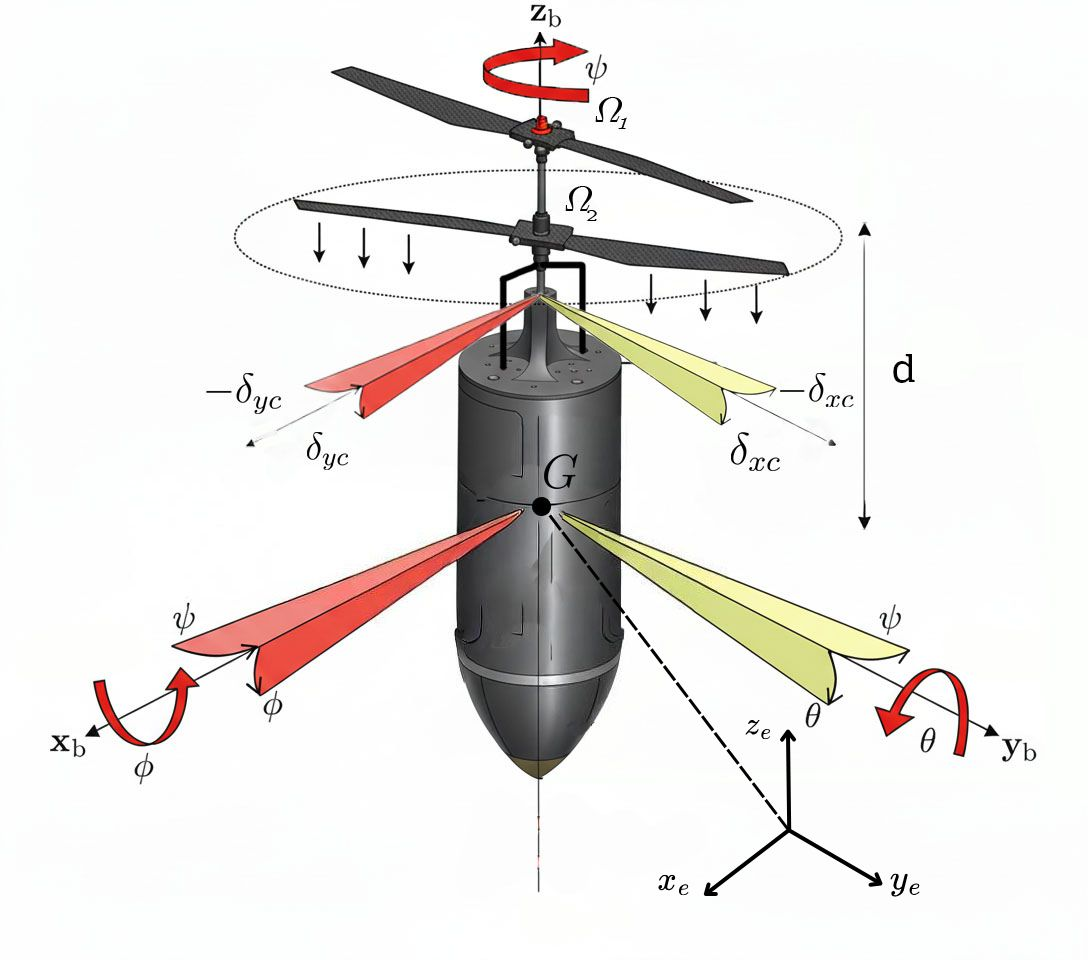
\includegraphics[width=8cm]{Thesis_ICD/figure5/coaxial.jpg}}
  \caption{Coaxial rotor vehicle configuration. }
  \label{coaxial_configuration}
\end{figure}


Two coordinate frames are defined: the inertial (Earth-fixed) frame
$\mathcal{E}(o_e, x_e, y_e, z_e)$ and the body-fixed frame
$\mathcal{B}(o_b, x_b, y_b, z_b)$ with origin at the center of gravity, as shown in
Figure~\ref{coaxial_configuration}. The UAV position in the inertial frame is
$p = [x, y, z]^T$, and its orientation is described by the Euler angles
$\eta = [\phi, \theta, \psi]^T$, representing roll, pitch, and yaw respectively.
The rotation matrix from the body frame to the inertial frame is
\begin{equation}
R =
\begin{bmatrix}
c_\theta c_\psi & s_\phi s_\theta c_\psi - c_\phi s_\psi & c_\phi s_\theta c_\psi + s_\phi s_\psi \\
c_\theta s_\psi & s_\phi s_\theta s_\psi + c_\phi c_\psi & c_\phi s_\theta s_\psi - s_\phi c_\psi \\
-s_\theta       & s_\phi c_\theta                         & c_\phi c_\theta
\end{bmatrix},
\end{equation}
where $s(\cdot)$ and $c(\cdot)$ denote the sine and cosine functions.

Applying Newton–Euler mechanics, the translational and rotational dynamics are
\begin{equation}
m\ddot{p} = RT - mg\begin{bmatrix}0\\0\\1\end{bmatrix} - K_p\dot{p} + F_{ext},
\qquad
J\ddot{\eta} = \Psi_\eta\tau - C(\eta,\dot{\eta}) - K_\eta\dot{\eta} + \tau_{ext},
\end{equation}
where $m$ is the vehicle mass, $J = \mathrm{diag}(I_x, I_y, I_z)$ is the inertia
matrix, $K_p$ and $K_\eta$ are positive-definite aerodynamic damping matrices,
$F_{ext}$ and $\tau_{ext}$ collect external disturbances and lumped uncertainties, and
$C(\eta, \dot{\eta})$ represents Coriolis and gyroscopic effects. The matrix
$\Psi_\eta$ maps Euler angle rates to body angular velocities.

The coaxial UAV has two rotors with angular speeds $\Omega_1$ (upper rotor) and
$\Omega_2$ (lower rotor). The swashplate deflections $\delta_{cx}$ and $\delta_{cy}$
regulate the cyclic pitch of the lower rotor. The resulting thrust vector and
control torques are
\begin{equation}
T =
\begin{bmatrix}
-k_\beta \sin\delta_{cy}\cos\delta_{cx}\,\Omega_2^2 \\
-k_\beta \sin\delta_{cx}\,\Omega_2^2 \\
k_\alpha\Omega_1^2 + k_\beta\cos\delta_{cx}\cos\delta_{cy}\,\Omega_2^2
\end{bmatrix},
\qquad
\tau =
\begin{bmatrix}
-dk_\beta\sin\delta_{cx}\,\Omega_2^2 \\
dk_\beta\sin\delta_{cy}\cos\delta_{cx}\,\Omega_2^2 \\
\gamma_1\Omega_1^2 - \gamma_2\Omega_2^2
\end{bmatrix},
\end{equation}
where $k_\alpha$ and $k_\beta$ are aerodynamic rotor coefficients, $d$ is the distance
from the center of gravity to the rotor hub, and $\gamma_1, \gamma_2$ are yaw
aerodynamic coefficients.

For small cyclic angles, the standard small-angle approximations
$\cos\delta_{cx} \approx \cos\delta_{cy} \approx 1$ and
$\sin\delta_{cx} \approx \delta_{cx}$, $\sin\delta_{cy} \approx \delta_{cy}$ hold.
Under this simplification, the six scalar equations of motion become
\begin{align}
\ddot{x} &= \frac{1}{m}\Big(Q_x(k_\alpha\Omega_1^2 + k_\beta\Omega_2^2) - K_x\dot{x} + F_x\Big), \label{eq:ddx}\\
\ddot{y} &= \frac{1}{m}\Big(Q_y(k_\alpha\Omega_1^2 + k_\beta\Omega_2^2) - K_y\dot{y} + F_y\Big), \label{eq:ddy}\\
\ddot{z} &= \frac{1}{m}\Big(Q_z(k_\alpha\Omega_1^2 + k_\beta\Omega_2^2) - K_z\dot{z} - mg + F_z\Big), \label{eq:ddz}\\
\ddot{\phi}   &= \frac{1}{I_x}\Big((I_y-I_z)\dot{\theta}\dot{\psi} - K_\phi\dot{\phi} - dk_\beta\delta_{cx}\Omega_2^2 + \tau_\phi\Big), \label{eq:ddphi}\\
\ddot{\theta} &= \frac{1}{I_y}\Big((I_z-I_x)\dot{\phi}\dot{\psi}  - K_\theta\dot{\theta} + dk_\beta\delta_{cy}\Omega_2^2 + \tau_\theta\Big), \label{eq:ddtheta}\\
\ddot{\psi}   &= \frac{1}{I_z}\Big((I_x-I_y)\dot{\phi}\dot{\theta} - K_\psi\dot{\psi} + \gamma_1\Omega_1^2 - \gamma_2\Omega_2^2 + \tau_\psi\Big), \label{eq:ddpsi}
\end{align}
where $Q_x = \cos\phi\sin\theta\cos\psi + \sin\phi\sin\psi$,
$Q_y = \cos\phi\sin\theta\sin\psi - \sin\phi\cos\psi$, and
$Q_z = \cos\phi\cos\theta$ are the direction cosines that project the total thrust
onto the inertial axes.

The physical actuator variables $\Omega_1$, $\Omega_2$, $\delta_{cx}$, $\delta_{cy}$
are mapped to virtual control inputs $T_z$, $\tau_\phi$, $\tau_\theta$, $\tau_\psi$
through the invertible relations
\begin{align}
\Omega_1^2 &= \frac{\gamma_2 T_z - k_\beta\tau_\psi}{k_\alpha\gamma_2 + k_\beta\gamma_1}, \qquad
\Omega_2^2  = \frac{\gamma_1 T_z - k_\alpha\tau_\psi}{k_\alpha\gamma_2 + k_\beta\gamma_1}, \label{eq:omega}\\
\delta_{cx} &= -\frac{\tau_\phi}{dk_\beta\Omega_2^2}, \qquad
\delta_{cy}  = \frac{\tau_\theta}{dk_\beta\Omega_2^2}. \label{eq:delta}
\end{align}
This inversion is valid provided $\Omega_2 \neq 0$, which holds during normal flight.

\subsection*{Multi-UAV model with actuator faults}

For a formation of $N$ coaxial UAVs, the equations above are extended to each agent
$i \in \{1, \ldots, N\}$. The total thrust input of the $i$-th UAV is decomposed as
\begin{equation}
u_{x,i}^a = Q_{x,i}\,u_{1,i}^a, \quad
u_{y,i}^a = Q_{y,i}\,u_{1,i}^a, \quad
u_{z,i}^a = Q_{z,i}\,u_{1,i}^a,
\end{equation}
where $u_{1,i}^a = \sqrt{(u_{x,i}^a)^2 + (u_{y,i}^a)^2 + (u_{z,i}^a)^2}$ is the
total thrust magnitude, and $Q_{x,i}$, $Q_{y,i}$, $Q_{z,i}$ are the direction cosines
of the $i$-th UAV evaluated at its current attitude. The equations of motion of the
$i$-th agent, incorporating the lumped nonlinearities $\Lambda_{\ell,i}$ and bounded
disturbances $d_{\ell,i}$, take the form
\begin{align}
\ddot{x}_i     &= u_{x,i}^a + \Lambda_{x,i} + d_{x,i}, \label{eq:xi}\\
\ddot{y}_i     &= u_{y,i}^a + \Lambda_{y,i} + d_{y,i}, \label{eq:yi}\\
\ddot{z}_i     &= u_{z,i}^a + \Lambda_{z,i} + d_{z,i}, \label{eq:zi}\\
\ddot{\phi}_i   &= u_{2,i}^a + \Lambda_{\phi,i}   + d_{\phi,i}, \label{eq:phii}\\
\ddot{\theta}_i &= u_{3,i}^a + \Lambda_{\theta,i} + d_{\theta,i}, \label{eq:thetai}\\
\ddot{\psi}_i   &= u_{4,i}^a + \Lambda_{\psi,i}   + d_{\psi,i}, \label{eq:psii}
\end{align}
where $\Lambda_{\ell,i}$ absorbs the known nonlinear terms from
\eqref{eq:ddx}--\eqref{eq:ddpsi} (Coriolis coupling, gravity, damping), and
$d_{\ell,i}$ is a bounded external disturbance, $|d_{\ell,i}| \leq \bar{d}_{\ell}$,
for $\ell \in \{x, y, z, \phi, \theta, \psi\}$.

In practical flight, actuators are subject to faults that degrade their output. Each
actuator $j \in \{1, 2, 3, 4\}$ of UAV $i$ is modeled by
\begin{equation}
u_{j,i}^a(t) = \rho_{j,i}(t)\,u_{j,i}(t) + \zeta_{j,i}(t),
\label{eq:fault}
\end{equation}
where $u_{j,i}(t)$ is the commanded input, $\rho_{j,i}(t) \in [\underline{\rho}, 1]$
with $\underline{\rho} > 0$ is an unknown time-varying effectiveness factor, and
$\zeta_{j,i}(t)$ is an unknown bounded additive bias, $|\zeta_{j,i}| \leq
\bar{\zeta}$. The case $\rho_{j,i} = 1$ and $\zeta_{j,i} = 0$ corresponds to a
fault-free actuator, while $0 < \underline{\rho} \leq \rho_{j,i} < 1$ represents
a partial loss of effectiveness, and $\zeta_{j,i} \neq 0$ represents a bias fault.
The assumption $\underline{\rho} > 0$ ensures that no actuator fails completely.

Substituting the fault model \eqref{eq:fault} into the UAV dynamics, the position
and attitude subsystems of the $i$-th UAV take the compact vector forms
\begin{align}
\ddot{p}_i &= \rho_{p,i}\,u_{p,i} + Q_{p,i}\,\zeta_{p,i} + \Lambda_{p,i} + d_{p,i}, \label{eq:pos_fault}\\
\ddot{\eta}_i &= \rho_{\eta,i}\,u_{\eta,i} + \zeta_{\eta,i} + \Lambda_{\eta,i} + d_{\eta,i}, \label{eq:att_fault}
\end{align}
where $p_i = [x_i, y_i, z_i]^T$, $\eta_i = [\phi_i, \theta_i, \psi_i]^T$,
$\rho_{p,i} = \mathrm{diag}\{\rho_{1,i}, \rho_{1,i}, \rho_{1,i}\}$,
$\rho_{\eta,i} = \mathrm{diag}\{\rho_{2,i}, \rho_{3,i}, \rho_{4,i}\}$, and
$Q_{p,i} = \mathrm{diag}\{Q_{x,i}, Q_{y,i}, Q_{z,i}\}$.

\begin{remark}
Throughout this chapter, the index $i \in \{1, \ldots, N\}$ refers to the UAV
agent, the index $j \in \{1, 2, 3, 4\}$ refers to the actuator channel, and
$\ell \in \{x, y, z, \phi, \theta, \psi\}$ refers to the state coordinate. The
compact subsystem notation in \eqref{eq:pos_fault}--\eqref{eq:att_fault} will
be used throughout the control design and stability analysis.
\end{remark}
\section{Control Objective}
\label{sec5:control_objective}

This chapter focuses on designing a distributed fault-tolerant formation controller for a group of $N$ coaxial rotor UAVs. The fleet consists of $N$ followers and one virtual leader, indexed by 0, which provides the reference trajectory for the entire formation. The primary goal is to develop a control strategy that enables all follower UAVs to track the virtual leader while maintaining a prescribed geometric formation, even in the presence of unmodeled dynamics, external disturbances, switching communication topologies, and faults in actuators.

To achieve this, the overall control objective is decomposed into two interconnected parts:

\textbf{1) Formation Tracking Objective:}
The first objective is to design a distributed protocol such that the desired trajectories of all follower UAVs, denoted by $p_i^s(t)$, converge to the virtual leader's trajectory $p_0(t)$ while maintaining the specified formation pattern. Let $p_d(t) = p_0(t)$ be the desired trajectory provided by the leader, and let $\tilde{p}_{i,d}$ be the desired constant position offset for the $i$-th UAV relative to the leader. The objective is to ensure that for any bounded initial conditions, there exist small positive constants $\epsilon_p$ and $\epsilon_v$ such that the formation tracking errors are ultimately bounded. Specifically, for all $i \in \{1, \dots, N\}$, the objective trajectories must satisfy:
\begin{equation}
    \lim_{t \to \infty} \| p_i^s(t) - p_d(t) - \tilde{p}_{i,d} \| \le \epsilon_p, \quad \lim_{t \to \infty} \| \dot{p}_i^s(t) - \dot{p}_d(t) \| \le \epsilon_v
    \label{eq:formation_objective}
\end{equation}
This must be achieved in a fixed time, ensuring rapid and predictable convergence to the desired formation structure. Similarly for the yaw angle we have:
\begin{equation}
\lim_{t \to \infty} | \psi(t) - \psi_d(t) | \le \epsilon_{\psi}
    \label{eq:formation_objectiveyaw}
\end{equation}

\textbf{2) Individual UAV Tracking Objective:}
The second objective is to design a robust, fault-tolerant controller for each individual coaxial UAV to ensure that its actual state trajectories, $p_i(t)$ and $\eta_i(t)$, accurately track the desired trajectories, $p_i^s(t)$ and $\eta_i^s(t)$, generated by the formation controller. This must be accomplished despite the presence of lumped uncertainties, disturbances, and faults. For any bounded initial conditions, the individual tracking errors must be guaranteed to converge to a small neighborhood of the origin in a fixed time. That is, there exist small positive constants $\epsilon_{p,i}$ and $\epsilon_{\eta,i}$ such that:
\begin{equation}
    \lim_{t \to T_{max}} \| p_i(t) - p_i^s(t) \| \le \epsilon_{p,i}, \quad \lim_{t \to T_{max}} \| \dot{p}_i(t) - \dot{p}_i^s(t) \| \le \epsilon_{v,i}, \quad    \lim_{t \to T_{max}} \| \psi_i(t) - \psi_i^s(t) \| \le \epsilon_{\psi,i}
\end{equation}
where $T_{max}$ is a settling time that is independent of the initial tracking errors. Satisfying this objective ensures the physical execution of the formation commands generated by the higher-level controller.

\section{Control Design}
\label{sec5:control_design}

To achieve the objectives stated in Section~\ref{sec5:control_objective}, a
hierarchical two-layer control architecture is proposed. The outer layer is a
distributed formation protocol that generates, for each follower UAV, a desired
objective trajectory $p_i^s(t)$ based solely on local neighbor information. The
inner layer is an individual fixed-time fault-tolerant controller that drives each
UAV's actual state to track its assigned objective trajectory, despite actuator
faults and lumped uncertainties. The unknown nonlinear terms are approximated
online by a Self-Structuring Neural Network (SSNN), which adapts its own
architecture in real time to match the complexity of the uncertainty.

The following assumptions are required for the controller design.

\begin{assumption}
\label{assum:leader}
The virtual leader's trajectory $p_d(t)$ and its first and second derivatives are
bounded. Specifically, there exist positive constants $R_p$ and $R_\chi$ such that
$\|\ddot{p}_d\| \leq R_p$ and $\|\ddot{\eta}_d\| \leq R_\chi$. Furthermore, all
system states are available for measurement.
\end{assumption}

\begin{assumption}
\label{assum:disturbance}
The external disturbances $d_{\ell,i}(t)$ and the additive bias faults
$\zeta_{j,i}(t)$ are bounded, i.e., $|d_{\ell,i}(t)| \leq \bar{d}_\ell$ and
$|\zeta_{j,i}(t)| \leq \bar{\zeta}$, where $\bar{d}_\ell$ and $\bar{\zeta}$ are
positive constants.
\end{assumption}

%-----------------------------------------------------------------------
\subsection{Formation Error Definition}
\label{sec5:formation_error}
%-----------------------------------------------------------------------

The formation error for the $i$-th UAV is defined using only the information
available from its local neighborhood $\mathcal{N}_i(t)$. Let $p_i^s \in
\mathbb{R}^3$ denote the objective trajectory to be designed for UAV $i$, and
let $h_i \in \mathbb{R}^3$ be the constant desired position offset of UAV $i$
relative to the virtual leader. The formation tracking error is defined as
\begin{equation}
    \epsilon_{p,i} = \sum_{j \in \mathcal{N}_i(t)} a_{ij}^{\sigma(t)}
    \left[(p_i^s - h_i) - (p_j^s - h_j)\right]
    + b_i^{\sigma(t)}(p_i^s - h_i - p_d),
    \label{eq:form_error_local}
\end{equation}
where $a_{ij}^{\sigma(t)}$ are the adjacency weights and $b_i^{\sigma(t)}$
indicates connectivity to the virtual leader. Using the stacked notation
$\epsilon_p = [\epsilon_{p,1}^T, \ldots, \epsilon_{p,N}^T]^T \in \mathbb{R}^{3N}$,
$p^s = [p_1^{sT}, \ldots, p_N^{sT}]^T$, and $\tilde{h} = [h_1^T, \ldots,
h_N^T]^T$, equation~\eqref{eq:form_error_local} takes the compact matrix form
\begin{equation}
    \epsilon_p = \mathbf{H}_{\sigma(t)} \otimes I_3
    \left(p^s - \tilde{h} - p_d \otimes \mathbf{1}_N\right),
    \label{eq:form_error_matrix}
\end{equation}
where $\mathbf{H}_{\sigma(t)} = \mathbf{L}_{\sigma(t)} + \mathbf{B}_{\sigma(t)}$
is the augmented Laplacian matrix. Under Assumption~\ref{assum:graph},
$\mathbf{H}_{\sigma(t)}$ is symmetric positive definite for all $t \geq 0$, with
minimum eigenvalue $\lambda_{\min} > 0$.

Taking the time derivative of \eqref{eq:form_error_matrix}, and noting that
$h_i$ is constant, the formation error dynamics are
\begin{equation}
    \dot{\epsilon}_p = \left(\mathbf{H}_{\sigma(t)} \otimes I_3\right)
    \left(\dot{p}^s - \dot{p}_d \otimes \mathbf{1}_N\right).
    \label{eq:form_error_dyn}
\end{equation}

To facilitate the control design, an auxiliary variable is introduced:
\begin{equation}
    \chi_{p,i} = \dot{\epsilon}_{p,i} + k_p \epsilon_{p,i},
    \label{eq:chi_def}
\end{equation}
where $k_p > 0$ is a positive design constant. In stacked form,
$\chi_p = [\chi_{p,1}^T, \ldots, \chi_{p,N}^T]^T$, and the error dynamics
can be rewritten as $\dot{\epsilon}_p = \chi_p - k_p \epsilon_p$.

%-----------------------------------------------------------------------
\subsection{Distributed Formation Controller}
\label{sec5:formation_controller}
%-----------------------------------------------------------------------

The distributed formation controller generates the objective trajectory
$p_i^s(t)$ for each UAV. The dynamics of the objective trajectory are governed
by the protocol
\begin{equation}
    \dot{p}_i^s = u_{p,i}^s,
    \label{eq:obj_traj_dyn}
\end{equation}
where $u_{p,i}^s \in \mathbb{R}^3$ is the auxiliary formation control input to
be designed. The time derivative of $\chi_{p,i}$ yields
\begin{equation}
    \dot{\chi}_p = \left(\mathbf{H}_{\sigma(t)} \otimes I_3\right)
    \left(\dot{u}_p^s - \ddot{p}_d \otimes \mathbf{1}_N\right)
    + k_p \dot{\epsilon}_p,
\end{equation}
where $u_p^s = [u_{p,1}^{sT}, \ldots, u_{p,N}^{sT}]^T$. The auxiliary formation
control law is designed as
\begin{equation}
    u_{p,i}^s = -k_\chi \chi_{p,i},
    \label{eq:formation_law}
\end{equation}
where $k_\chi > 0$ is a positive design constant.

\begin{remark}
The formation control law \eqref{eq:formation_law} requires only the local
formation error $\epsilon_{p,i}$ and its derivative, both of which are computed
from the states of UAV $i$ and its direct neighbors. This ensures the strictly
distributed nature of the protocol.
\end{remark}

\begin{theorem}
\label{thm:formation}
Under Assumption~\ref{assum:leader} and Assumption~\ref{assum:graph}, the
distributed formation protocol \eqref{eq:formation_law} guarantees that the
formation errors $\epsilon_{p,i}$ and $\chi_{p,i}$ are uniformly ultimately
bounded (UUB). Specifically, the objective trajectories $p_i^s$ converge such
that $\lim_{t \to \infty} \|p_i^s - p_d - h_i\| \leq \epsilon_p$ for some
small positive constant $\epsilon_p$.
\end{theorem}

\begin{proof}
Consider the Lyapunov function candidate
\begin{equation}
    V_1 = \frac{1}{2} \epsilon_p^T \epsilon_p + \frac{1}{2} \chi_p^T \chi_p.
    \label{eq:V1}
\end{equation}
Taking the time derivative and substituting $\dot{\epsilon}_p = \chi_p - k_p
\epsilon_p$ yields
\begin{equation}
    \dot{V}_1 = \epsilon_p^T(\chi_p - k_p \epsilon_p) + \chi_p^T \dot{\chi}_p.
\end{equation}
Substituting the control law \eqref{eq:formation_law} and noting that
$\dot{u}_p^s = -k_\chi \dot{\chi}_p$ gives
\begin{align}
    \dot{V}_1 &= -k_p \|\epsilon_p\|^2 + \epsilon_p^T \chi_p
    - k_\chi \chi_p^T (\mathbf{H}_{\sigma(t)} \otimes I_3) \chi_p \nonumber \\
    &\quad - \chi_p^T (\mathbf{H}_{\sigma(t)} \otimes I_3)
    (\ddot{p}_d \otimes \mathbf{1}_N)
    + k_p \|\chi_p\|^2 - k_p^2 \chi_p^T \epsilon_p.
    \label{eq:V1dot_expanded}
\end{align}
Applying Lemma~\ref{lemma3} to the cross terms with positive constants
$a_1, a_2, a_3 > 0$:
\begin{align}
    \epsilon_p^T \chi_p &\leq \frac{1}{2a_1}\|\epsilon_p\|^2
    + \frac{a_1}{2}\|\chi_p\|^2, \label{eq:Y1}\\
    -k_p^2 \chi_p^T \epsilon_p &\leq \frac{k_p^2}{2a_2}\|\epsilon_p\|^2
    + \frac{a_2 k_p^2}{2}\|\chi_p\|^2, \label{eq:Y2}\\
    -\chi_p^T (\mathbf{H}_{\sigma(t)} \otimes I_3)(\ddot{p}_d \otimes
    \mathbf{1}_N) &\leq \frac{1}{2a_3}\|\chi_p\|^2 + \Xi_1,
    \label{eq:Y3}
\end{align}
where $\Xi_1 = \frac{a_3}{2}\|\mathbf{H}_{\sigma(t)}\|^2 N R_p^2$ is a
positive constant. Since $\mathbf{H}_{\sigma(t)}$ is positive definite with
smallest eigenvalue $\lambda_{\min}$:
\begin{equation}
    -k_\chi \chi_p^T (\mathbf{H}_{\sigma(t)} \otimes I_3) \chi_p
    \leq -k_\chi \lambda_{\min} \|\chi_p\|^2.
    \label{eq:Y4}
\end{equation}
Substituting \eqref{eq:Y1}--\eqref{eq:Y4} into \eqref{eq:V1dot_expanded}:
\begin{equation}
    \dot{V}_1 \leq -Q_p \|\epsilon_p\|^2 - T_p \|\chi_p\|^2 + \Xi_1,
    \label{eq:V1dot_final}
\end{equation}
where
\begin{equation}
    Q_p = k_p - \frac{1}{2a_1} - \frac{k_p^2}{2a_2}, \qquad
    T_p = k_\chi \lambda_{\min} - \frac{a_1}{2} - \frac{a_2 k_p^2}{2}
    - k_p - \frac{1}{2a_3}.
\end{equation}
By selecting $k_p$, $k_\chi$, $a_1$, $a_2$, $a_3$ such that $Q_p > 0$ and
$T_p > 0$, and letting $\rho = \min\{2Q_p, 2T_p\}$, equation
\eqref{eq:V1dot_final} becomes
\begin{equation}
    \dot{V}_1 \leq -\rho V_1 + \Xi_1.
    \label{eq:V1_uub}
\end{equation}
The solution to this differential inequality satisfies
$V_1(t) \leq (V_1(0) - \Xi_1/\rho)e^{-\rho t} + \Xi_1/\rho$,
which implies $\lim_{t \to \infty} V_1(t) \leq \Xi_1/\rho$. Since $V_1$ is
positive definite in $\epsilon_p$ and $\chi_p$, both are UUB, and the formation
errors converge to a bounded neighborhood of the origin of radius
$\sqrt{2\Xi_1/\rho}$. This completes the proof.
\end{proof}

%-----------------------------------------------------------------------
\subsection{Self-Structuring Neural Network Design}
\label{sec5:ssnn}
%-----------------------------------------------------------------------

Once $p_i^s$ is generated by the formation controller, each UAV must track it
despite the presence of lumped uncertainties, disturbances, and actuator faults.
Both the position and attitude subsystems of the $i$-th UAV, from
\eqref{eq:pos_fault}--\eqref{eq:att_fault}, can be written in a unified generic
form
\begin{equation}
    \ddot{q}_i = \rho_i u_i + \Delta_i(t),
    \label{eq:generic_subsystem}
\end{equation}
where $q_i$ stands for either $p_i$ or $\eta_i$, $u_i$ is the control input,
$\rho_i \geq \underline{\rho} > 0$ is the unknown effectiveness factor, and
$\Delta_i(t)$ is the total lumped uncertainty defined as
\begin{equation}
    \Delta_i(t) = Q_i(\cdot)\zeta_i + \Lambda_i + d_i(t).
    \label{eq:lumped}
\end{equation}
The function $\Delta_i(t)$ is unknown and time-varying, encompassing the
additive fault bias, the nonlinear aerodynamic coupling terms, and the external
disturbance. To handle it without prior knowledge or offline training, an
Adaptive Self-Structuring Neural Network (SSNN) is employed to approximate it
online \cite{SSNN1, SSNN_Ref2}.

The SSNN approximates $\Delta_i(t)$ as
\begin{equation}
    \Delta_i(t) = W_i^{*T} \Phi_i(Z_i) + \delta_i(Z_i),
    \label{eq:ssnn_approx}
\end{equation}
where $W_i^* \in \mathbb{R}^{M_i}$ is the ideal weight vector,
$\Phi_i(Z_i) = [\phi_1(Z_i), \ldots, \phi_{M_i}(Z_i)]^T$ is the vector of
Gaussian basis functions with $Z_i = [q_i^T, \dot{q}_i^T]^T$ as the network
input, $M_i$ is the current number of hidden neurons, and $\delta_i$ is the
bounded approximation error satisfying $\|\delta_i\| \leq \bar{\delta}$.

The key advantage of the SSNN over a fixed-structure neural network is its
ability to dynamically adjust the number of hidden neurons during operation.
This is governed by two mechanisms.

\subsubsection*{Neuron growing}
A new neuron is added when the maximum activation of the existing neurons falls
below a threshold, indicating that the current network is insufficient to cover
the operating region. Specifically, if $h_{\max}(t) = \max_k h_k(Z_i) < G_{\text{th}}$,
where $G_{\text{th}} \in (0,1)$ is a predefined growing threshold, a new neuron
is inserted with center and width initialized as
\begin{equation}
    c_{\text{new}} = \frac{Z_i + c_j}{2}, \qquad
    b_{\text{new}} = b_j, \qquad W_{\text{new}} = 0,
    \label{eq:neuron_split}
\end{equation}
where $c_j$ and $b_j$ are the center and width of the least-activated existing
neuron, and $h_k(Z_i) = \exp(-\|Z_i - c_k\|^2 / b_k^2)$ is the Gaussian
activation of the $k$-th neuron.

\subsubsection*{Neuron pruning}
To prevent unnecessary growth and limit onboard computational cost, neurons
that remain persistently inactive are removed. A pruning index $I_k$ is
maintained for each neuron and updated as
\begin{equation}
    I_k = \begin{cases}
        e^{-\nu} I_{k}^{\text{prev}}, & \text{if } h_k(Z_i) < P_{\text{th}}, \\
        I_{k}^{\text{prev}},           & \text{otherwise},
    \end{cases}
    \label{eq:pruning_index}
\end{equation}
where $P_{\text{th}} \in (0,1)$ is a pruning activity threshold, $\nu > 0$ is
a decay constant, and $I_k^{\text{prev}}$ is the index from the previous time
step. A neuron is removed when $I_k < I_{\text{th}}$, where $I_{\text{th}}$ is
a minimum index threshold.

The weight vector is updated online by the following adaptive law:
\begin{equation}
    \dot{\hat{W}}_i = \Gamma_i s_i \Phi_i(Z_i) - \sigma_i \Gamma_i \hat{W}_i,
    \label{eq:weight_law}
\end{equation}
where $\hat{W}_i$ is the estimated weight vector, $\Gamma_i > 0$ is a
positive-definite learning rate matrix, $\sigma_i > 0$ is a leakage term that
prevents parameter drift, and $s_i$ is the sliding variable defined in the
next subsection. The estimation error is $\tilde{W}_i = W_i^* - \hat{W}_i$.

\begin{remark}
Unlike fixed-structure RBFNNs, the SSNN does not require the number of neurons
to be specified in advance. In dynamic swarm environments where the complexity
of aerodynamic coupling between coaxial agents varies continuously during
flight, the SSNN grows its structure when the uncertainty changes rapidly and
prunes it when the operation stabilizes, maintaining high approximation accuracy
while keeping the computational burden minimal for onboard processors.
\end{remark}

%-----------------------------------------------------------------------
\subsection{Fixed-Time Fault-Tolerant Control Law}
\label{sec5:control_law}
%-----------------------------------------------------------------------

\subsubsection{Fixed-time sliding surface}

For each UAV $i$, the tracking error with respect to its objective trajectory
is defined as
\begin{equation}
    e_{1,i} = q_i - q_i^s, \qquad e_{2,i} = \dot{q}_i - \dot{q}_i^s,
    \label{eq:tracking_errors}
\end{equation}
where $q_i^s$ stands for either $p_i^s$ or $\eta_i^s$. A fixed-time sliding
surface is defined as
\begin{equation}
    s_i = e_{2,i} + \alpha_1 |e_{1,i}|^{\rho_1} \text{sgn}(e_{1,i})
        + \alpha_2 |e_{1,i}|^{\rho_2} \text{sgn}(e_{1,i}),
    \label{eq:sliding_surface}
\end{equation}
where $\alpha_1, \alpha_2 > 0$, $0 < \rho_1 < 1$, and $\rho_2 > 1$. When the
system state reaches the manifold $s_i = 0$, the error dynamics satisfy
$\dot{e}_{1,i} = -\alpha_1|e_{1,i}|^{\rho_1}\text{sgn}(e_{1,i})
-\alpha_2|e_{1,i}|^{\rho_2}\text{sgn}(e_{1,i})$, which is a standard fixed-time
stable system whose settling time is bounded by
$T_s \leq 1/(\alpha_1(1-\rho_1)) + 1/(\alpha_2(\rho_2-1))$, independent of
$e_{1,i}(0)$ \cite{Polyakov2012}.

Taking the time derivative of \eqref{eq:sliding_surface} and substituting the
system dynamics \eqref{eq:generic_subsystem}:
\begin{align}
    \dot{s}_i &= \ddot{q}_i - \ddot{q}_i^s
    + \alpha_1 \rho_1 |e_{1,i}|^{\rho_1-1} e_{2,i}
    + \alpha_2 \rho_2 |e_{1,i}|^{\rho_2-1} e_{2,i} \nonumber \\
    &= \rho_i u_i + \Delta_i(t) - \ddot{q}_i^s
    + \alpha_1 \rho_1 |e_{1,i}|^{\rho_1-1} e_{2,i}
    + \alpha_2 \rho_2 |e_{1,i}|^{\rho_2-1} e_{2,i}.
    \label{eq:sdot}
\end{align}
Defining the total compounded uncertainty as
\begin{equation}
    D_i = \Delta_i(t) - \ddot{q}_i^s
    + \alpha_1 \rho_1 |e_{1,i}|^{\rho_1-1} e_{2,i}
    + \alpha_2 \rho_2 |e_{1,i}|^{\rho_2-1} e_{2,i},
    \label{eq:Di}
\end{equation}
the sliding dynamics simplify to
\begin{equation}
    \dot{s}_i = \rho_i u_i + D_i.
    \label{eq:sliding_dyn}
\end{equation}
The function $D_i$ is unknown and is approximated by the SSNN:
$\hat{D}_i = \hat{W}_i^T \Phi_i(Z_i)$.

\subsubsection{Position controller}

The position tracking error is $r_{p,i} = p_i - p_i^s$ and $\dot{r}_{p,i} =
\dot{p}_i - \dot{p}_i^s$. The sliding surface for the position subsystem is \cite{formation_control_fault1}
\begin{equation}
    s_{p,i} = \dot{r}_{p,i}
    + \alpha_{p1} |r_{p,i}|^{\rho_{p1}} \text{sgn}(r_{p,i})
    + \alpha_{p2} |r_{p,i}|^{\rho_{p2}} \text{sgn}(r_{p,i}),
    \label{eq:sp}
\end{equation}
where $\alpha_{p1}, \alpha_{p2} > 0$, $0 < \rho_{p1} < 1$, $\rho_{p2} > 1$.
The position control law is designed as
\begin{equation}
    u_{p,i} = -k_{p1} s_{p,i} - k_{p2} |s_{p,i}|^\gamma \text{sgn}(s_{p,i})
    - \hat{W}_{p,i}^T \Phi_{p,i}(Z_{p,i}),
    \label{eq:up}
\end{equation}
where $k_{p1}, k_{p2} > 0$ and $0 < \gamma < 1$ are design constants, and the
SSNN weight adaptation follows \eqref{eq:weight_law}. The total thrust input is
recovered as
\begin{equation}
    u_{i,1} = \|u_{p,i}\| = \sqrt{u_{x,i}^2 + u_{y,i}^2 + u_{z,i}^2}.
    \label{eq:u1}
\end{equation}
The desired roll and pitch angles are extracted from $u_{p,i}$ as
\begin{align}
    \varphi_i^s &= \arcsin\!\left(
    \frac{u_{x,i}\sin\psi_i^s - u_{y,i}\cos\psi_i^s}{\|u_{p,i}\|}
    \right), \label{eq:phi_des}\\
    \theta_i^s  &= \arctan\!\left(
    \frac{u_{x,i}\cos\psi_i^s + u_{y,i}\sin\psi_i^s}{u_{z,i}}
    \right), \label{eq:theta_des}
\end{align}
where $\psi_i^s$ is provided by the formation protocol analogously to
\eqref{eq:formation_law} applied to the yaw channel.

\subsubsection{Attitude controller}

The attitude tracking error is $r_{\eta,i} = \eta_i - \eta_i^s$ and
$\dot{r}_{\eta,i} = \dot{\eta}_i - \dot{\eta}_i^s$. The sliding surface for
the attitude subsystem is
\begin{equation}
    s_{\eta,i} = \dot{r}_{\eta,i}
    + \alpha_{\eta1} |r_{\eta,i}|^{\rho_{\eta1}} \text{sgn}(r_{\eta,i})
    + \alpha_{\eta2} |r_{\eta,i}|^{\rho_{\eta2}} \text{sgn}(r_{\eta,i}),
    \label{eq:schi}
\end{equation}
where $\alpha_{\eta1}, \alpha_{\eta2} > 0$, $0 < \rho_{\eta1} < 1$,
$\rho_{\eta2} > 1$. The attitude control law is
\begin{equation}
    u_{\eta,i} = -k_{\eta1} s_{\eta,i}
    - k_{\eta2} |s_{\eta,i}|^\gamma \text{sgn}(s_{\eta,i})
    - \hat{W}_{\eta,i}^T \Phi_{\eta,i}(Z_{\eta,i}),
    \label{eq:uchi}
\end{equation}
where $k_{\eta1}, k_{\eta2} > 0$ with weight adaptation following
\eqref{eq:weight_law}. The torque commands $\tau_\varphi$, $\tau_\theta$,
$\tau_\psi$ are recovered from $u_{\eta,i}$ through the inversion
\eqref{eq:omega}--\eqref{eq:delta}.

%-----------------------------------------------------------------------
\subsection{Stability Analysis}
\label{sec5:stability}
%-----------------------------------------------------------------------

\begin{theorem}
\label{thm:stability}
Consider the $i$-th coaxial UAV described by
\eqref{eq:pos_fault}--\eqref{eq:att_fault}, under
Assumptions~\ref{assum:graph}--\ref{assum:disturbance}, with the fixed-time
sliding surfaces \eqref{eq:sp} and \eqref{eq:schi}, the SSNN-based control
laws \eqref{eq:up} and \eqref{eq:uchi}, and the weight adaptation law
\eqref{eq:weight_law}. Then the tracking errors $e_{1,i}$ and $e_{2,i}$ of
both the position and attitude subsystems are practically fixed-time stable,
converging to a small neighborhood of the origin within the settling time
$T_{\max}$ defined in Lemma \eqref{lemma2}, independently of the initial conditions.
\end{theorem}

\begin{proof}
The proof is presented for the generic subsystem \eqref{eq:generic_subsystem},
covering both position ($\varpi = p$) and attitude ($\varpi = \eta$). Consider
the Lyapunov function candidate
\begin{equation}
    \mathcal{L}_i = \frac{1}{2} s_i^T s_i
    + \frac{1}{2} \tilde{W}_i^T \Gamma_i^{-1} \tilde{W}_i.
    \label{eq:Li}
\end{equation}
Taking the time derivative of \eqref{eq:Li}:
\begin{equation}
    \dot{\mathcal{L}}_i = s_i^T \dot{s}_i
    - \tilde{W}_i^T \Gamma_i^{-1} \dot{\hat{W}}_i.
    \label{eq:Lidot}
\end{equation}
Substituting the sliding dynamics \eqref{eq:sliding_dyn} and the SSNN
approximation \eqref{eq:ssnn_approx}:
\begin{equation}
    \dot{\mathcal{L}}_i = s_i^T \left(\rho_i u_i + W_i^{*T}\Phi_i + \delta_i\right)
    - \tilde{W}_i^T \Gamma_i^{-1} \dot{\hat{W}}_i.
    \label{eq:Lidot2}
\end{equation}
Substituting the control law \eqref{eq:up} (or \eqref{eq:uchi}):
\begin{align}
    \dot{\mathcal{L}}_i &\leq s_i^T \rho_i \left(-k_{1} s_i
    - k_{2}|s_i|^\gamma \text{sgn}(s_i)
    - \hat{W}_i^T \Phi_i\right) \nonumber\\
    &\quad + s_i^T\left(W_i^{*T}\Phi_i + \delta_i\right)
    - \tilde{W}_i^T \Gamma_i^{-1} \dot{\hat{W}}_i.
    \label{eq:Lidot3}
\end{align}
Since $\rho_i \geq \underline{\rho} > 0$, the first term satisfies
\begin{equation}
    -\rho_i k_1 \|s_i\|^2 \leq -\underline{\rho} k_1 \|s_i\|^2, \qquad
    -\rho_i k_2 \|s_i\|^{1+\gamma} \leq -\underline{\rho} k_2 \|s_i\|^{1+\gamma}.
\end{equation}
The cross term involving the NN weights is handled using the identity
$s_i^T \tilde{W}_i^T \Phi_i = s_i^T (W_i^* - \hat{W}_i)^T \Phi_i$, giving
\begin{equation}
    s_i^T W_i^{*T}\Phi_i - s_i^T \hat{W}_i^T \Phi_i \rho_i
    - \tilde{W}_i^T \Gamma_i^{-1} \dot{\hat{W}}_i.
\end{equation}
Substituting the weight adaptation law \eqref{eq:weight_law}:
\begin{equation}
    \tilde{W}_i^T \Gamma_i^{-1} \dot{\hat{W}}_i =
    \tilde{W}_i^T s_i \Phi_i - \sigma_i \tilde{W}_i^T \hat{W}_i.
\end{equation}
The unknown weight term $s_i^T W_i^{*T} \Phi_i$ is bounded using
Lemma~\ref{lemma3}:
\begin{equation}
    s_i^T W_i^{*T} \Phi_i \leq \frac{1}{2}\|s_i\|^2 \|\Phi_i\|^2
    + \frac{1}{2}\|W_i^*\|^2.
    \label{eq:young_nn}
\end{equation}
The leakage term is bounded by the triangle inequality:
\begin{equation}
    \sigma_i \tilde{W}_i^T \hat{W}_i
    \geq \frac{\sigma_i}{2}\|\tilde{W}_i\|^2 - \frac{\sigma_i}{2}\|W_i^*\|^2.
    \label{eq:leakage}
\end{equation}
The approximation error is bounded as $s_i^T \delta_i \leq \frac{1}{2}\|s_i\|^2
+ \frac{1}{2}\bar{\delta}^2$. Collecting all terms and choosing $k_1$ large
enough to absorb the quadratic $\|s_i\|^2$ terms, we obtain
\begin{equation}
    \dot{\mathcal{L}}_i \leq
    -\underline{\rho} k_2 \|s_i\|^{1+\gamma}
    - \frac{\sigma_i}{2}\|\tilde{W}_i\|^2 + C_i,
    \label{eq:Lidot_pre}
\end{equation}
where $C_i = \frac{\sigma_i}{2}\|W_i^*\|^2 + \frac{1}{2}\bar{\delta}^2$ is a
positive constant. Expressing \eqref{eq:Lidot_pre} in terms of $\mathcal{L}_i$:
since $\|s_i\|^{1+\gamma} = (\|s_i\|^2)^{(1+\gamma)/2} \geq
(2 \cdot \frac{1}{2}\|s_i\|^2)^{(1+\gamma)/2}$, and similarly for the weight
term, we obtain with $\rho_1 = (1+\gamma)/2 < 1$ and $\rho_2 = (3-\gamma)/2 > 1$:
\begin{equation}
    \dot{\mathcal{L}}_i \leq
    -\lambda_1 \mathcal{L}_i^{\rho_1}
    - \lambda_2 \mathcal{L}_i^{\rho_2} + \varpi_i,
    \label{eq:Lidot_fxt}
\end{equation}
where $\lambda_1 = \underline{\rho} k_2 \cdot 2^{\rho_1}$,
$\lambda_2 = \sigma_i \cdot 2^{\rho_2}$ (after appropriate algebraic
manipulation), and $\varpi_i = C_i$. By Lemma~\ref{lemma2}, inequality
\eqref{eq:Lidot_fxt} guarantees that $\mathcal{L}_i$ — and consequently
$s_i$ and $\tilde{W}_i$ — converge to a small residual set within the fixed
settling time $T_{\max}$ given in \eqref{lemma1}, independently of the initial
conditions. Once $s_i \to 0$, the tracking errors $e_{1,i}$ and $e_{2,i}$
converge to the origin on the sliding manifold within an additional fixed time
$T_s$. The total convergence time $T_{\max} + T_s$ remains bounded and
independent of initial conditions. This completes the proof.
\end{proof}

\begin{theorem}
\label{thm:full_system}
Under the same conditions as Theorem~\ref{thm:stability}, the composite
Lyapunov function for the entire $N$-agent coaxial UAV formation,
\begin{equation}
    V = V_1 + \sum_{i=1}^{N} \left(\mathcal{L}_{p,i} + \mathcal{L}_{\eta,i}\right),
    \label{eq:V_total}
\end{equation}
satisfies the practical fixed-time stability condition of Lemma~\ref{lemma2}.
Consequently, the formation errors $\epsilon_{p,i}$, position tracking errors
$r_{p,i}$, and attitude tracking errors $r_{\eta,i}$ all converge to small
bounded neighborhoods of the origin within a fixed settling time $T_{\max}$
that is independent of the initial conditions of any agent.
\end{theorem}

\begin{proof}
From Theorem~\ref{thm:formation}, $V_1$ satisfies \eqref{eq:V1_uub}, giving
$\dot{V}_1 \leq -\rho V_1 + \Xi_1$.
From Theorem~\ref{thm:stability}, each $\mathcal{L}_{p,i}$ and $\mathcal{L}_{\eta,i}$
satisfies \eqref{eq:Lidot_fxt}. Summing over all $N$ agents:
\begin{equation}
    \dot{V} \leq -\rho V_1 + \Xi_1
    - \sum_{i=1}^{N} \left(
    \lambda_1 \mathcal{L}_{p,i}^{\rho_1} + \lambda_2 \mathcal{L}_{p,i}^{\rho_2}
    + \lambda_1 \mathcal{L}_{\eta,i}^{\rho_1} + \lambda_2 \mathcal{L}_{\eta,i}^{\rho_2}
    \right) + N \varpi.
\end{equation}
Applying the power-mean inequality $\sum_{i=1}^N x_i^{\rho} \geq
N^{1-\rho}(\sum_{i=1}^N x_i)^{\rho}$ for $\rho \in (0,1)$ and a standard bound
for $\rho > 1$, and noting that $V_1 \leq V$, the overall derivative satisfies
\begin{equation}
    \dot{V} \leq -\Lambda_1 V^{\rho_1} - \Lambda_2 V^{\rho_2} + \Omega,
    \label{eq:Vdot_full}
\end{equation}
for appropriate positive constants $\Lambda_1$, $\Lambda_2$, and $\Omega$. By
Lemma~\ref{lemma2}, $V$ is practically fixed-time stable, completing the proof.
\end{proof}

\begin{remark}
The control laws \eqref{eq:up} and \eqref{eq:uchi} are implementable in a fully
distributed manner. Each UAV $i$ requires only its own state and the states of
its direct neighbors $\mathcal{N}_i(t)$ to compute $\epsilon_{p,i}$ and the
formation control signal. The SSNN runs entirely onboard each UAV with no
inter-agent communication of neural network weights.
\end{remark}

\begin{remark}
The $\text{sgn}(\cdot)$ function in \eqref{eq:up} and \eqref{eq:uchi} may
induce chattering in practice. This can be mitigated by replacing
$\text{sgn}(s_i)$ with the smooth approximation $s_i / (\|s_i\| + \epsilon_0)$
for a small $\epsilon_0 > 0$, which introduces a small additional bounded term
in the stability analysis without affecting the convergence result.
\end{remark}
\section{Simulation Results and Discussion}
\label{sec5:simulations}
To validate the effectiveness of the proposed distributed control strategy, a series of numerical simulations are conducted using MATLAB software. The formation consists of four coaxial rotor UAVs ($N=4$) tasked with following a virtual leader along a predefined trajectory while maintaining a square formation. The physical parameters for each identical coaxial UAV are set as follows: mass $m_i = 0.41$ kg, rotor distance $d = 0.067$ m, gravitational acceleration $g = 9.8$ m/s$^2$, and inertia matrix $J_i = \text{diag}(1.83 \times 10^{-3}, 1.83 \times 10^{-3}, 2.72 \times 10^{-4})$ kg$\cdot$m$^2$. To demonstrate the controller's ability to achieve formation from a dispersed state, each UAV begins at a different initial position. The communication topologies are allowed to switch among three possible configurations, as shown in Fig.~\ref{fig:topologies}. The switching signal $\sigma(t)$ dictates the active topology from the set, according to the following piecewise function:
\begin{equation}
\sigma(t) = 
\begin{cases}
    a, & \text{if } 0 \le t < 15s \\
    b, & \text{if } 15s \le t < 30s \\
    c, & \text{if } t \ge 30s
\end{cases}
\end{equation}

\begin{figure}[h!]
    \centering
    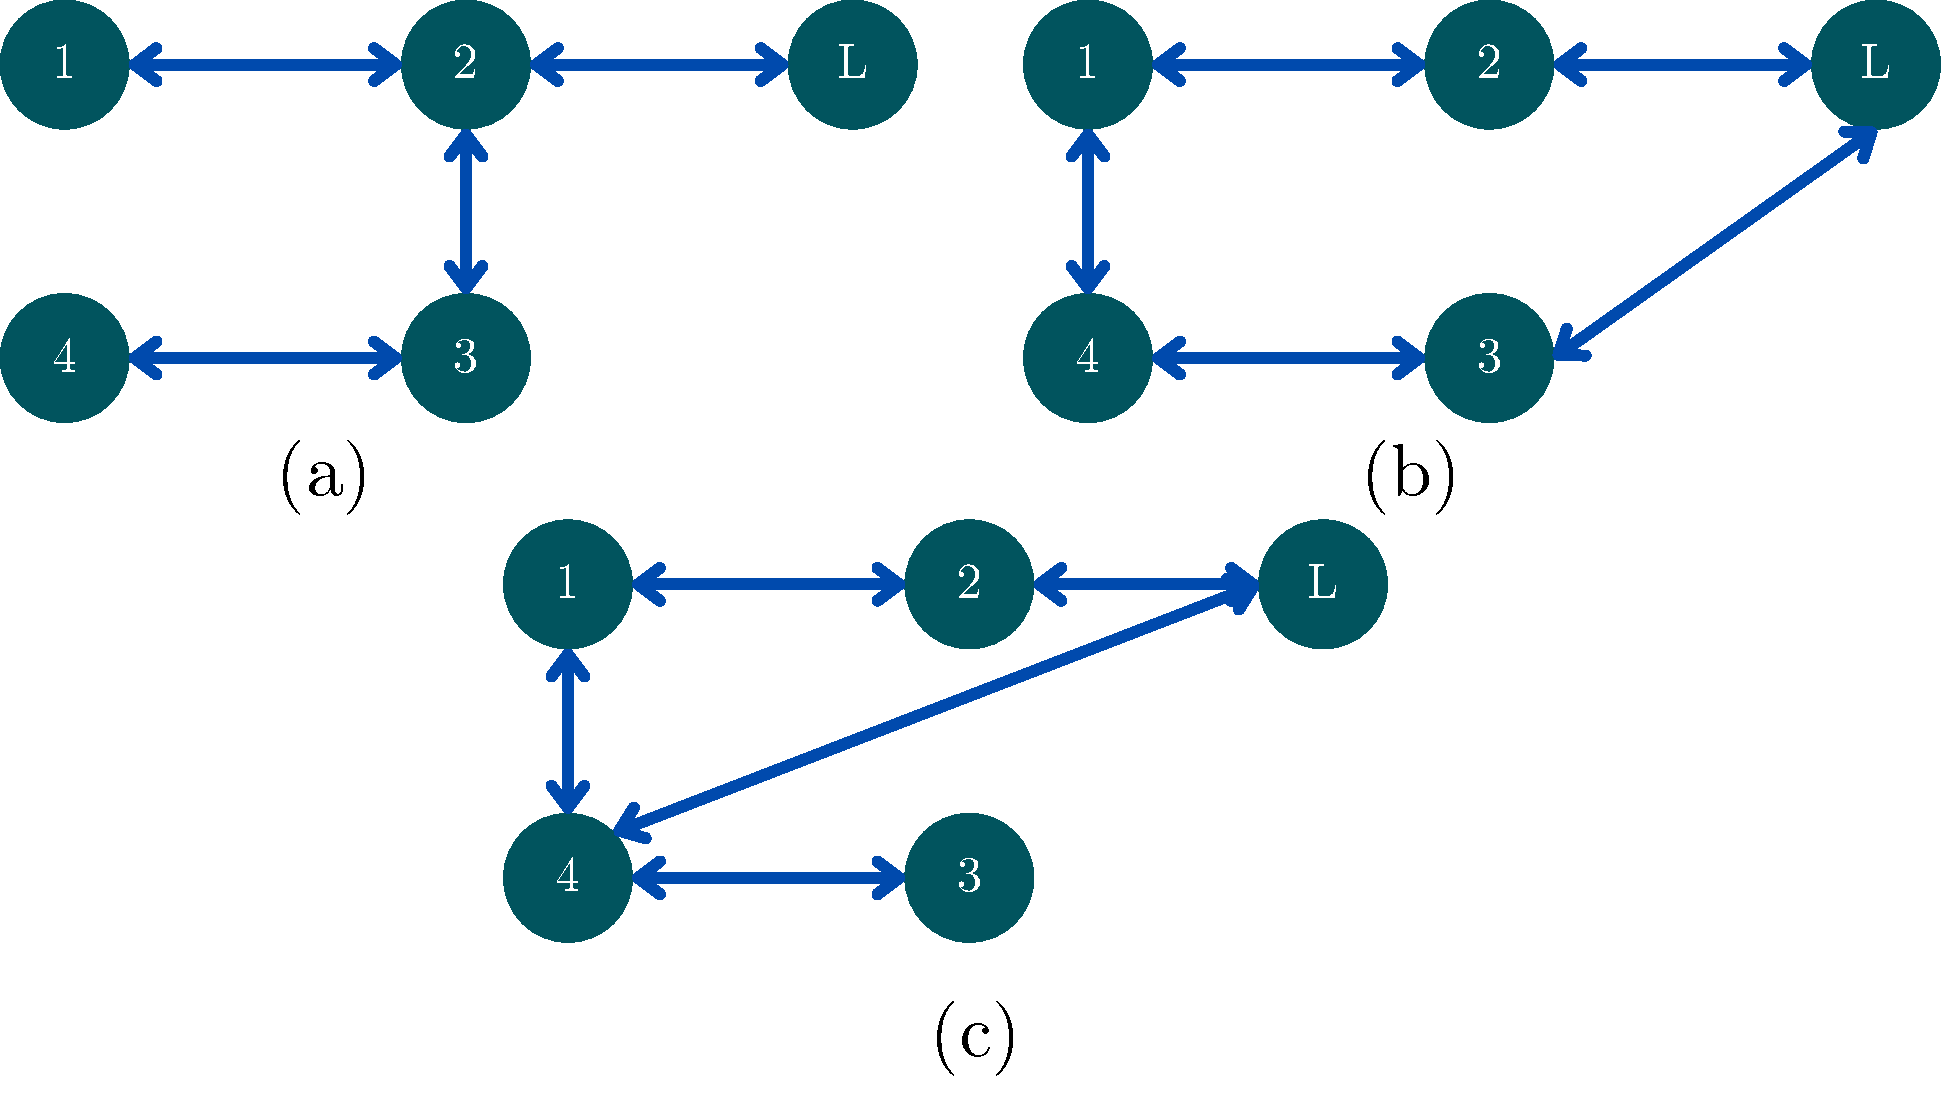
\includegraphics[width=0.8\textwidth]{Thesis_ICD/figure5/topologies.pdf}
    \caption{Possible communication topologies.}
    \label{fig:topologies}
\end{figure}

The reference trajectory for the virtual leader is set as $$p_d(t) = [2.5  \sin(0.1t), -2.5\cos(0.05t), 0.3  t + 2 sin(0.2t)]^T,$$ with a constant desired yaw angle of $\psi_d = 0$. To create a challenging environment, external sinusoidal disturbances are added to the position dynamics of all UAVs, and set as $d_i = 0.1\sin(t)$
To rigorously test the fault-tolerant capability of the designed control algorithm, actuator faults are injected into the first and third actuators of all UAVs simultaneously. The faults are designed to be time-varying to simulate challenging real-world failure modes. For each UAV $i \in \{1, 2, 3, 4\}$, the fault on the first actuator (main thrust) includes a partial loss of effectiveness, while the fault on the third actuator (a torque channel) includes both a loss of effectiveness and an additive bias. The specific fault profiles are modeled as follows:
\begin{equation}
u_{i,1}^{a} = 
\begin{cases}
    u_{i,1}, & t < 25s \\
    (0.8 + 0.1\sin(t))u_{i,1}, & 25s \le t < 35s \\
    (0.6 + 0.2\sin(t))u_{i,1}, & t \ge 35s
\end{cases}
\end{equation}
\begin{equation}
u_{i,3}^{a} = 
\begin{cases}
    u_{i,3}, & t < 25s \\
    u_{i,3} + 0.6, & 25s \le t < 35s \\
    (0.8 + 0.1\sin(t))u_{i,3} + 0.6, & t \ge 35s
\end{cases}
\end{equation}
These complex faults provide a test for the robustness and adaptability of the control system.

The results of the simulation under these combined challenges are presented and analyzed. Figure \ref{fig:3Dformation} shows the 3-D trajectories of the four follower UAVs. It is clear that despite starting from different locations and contending with faults and a switching communication network, all agents successfully converge to the desired square formation and track the leader's trajectory. This visually confirms the overall stability and effectiveness of the distributed control strategy.

\begin{figure}[h!]
    \centering
    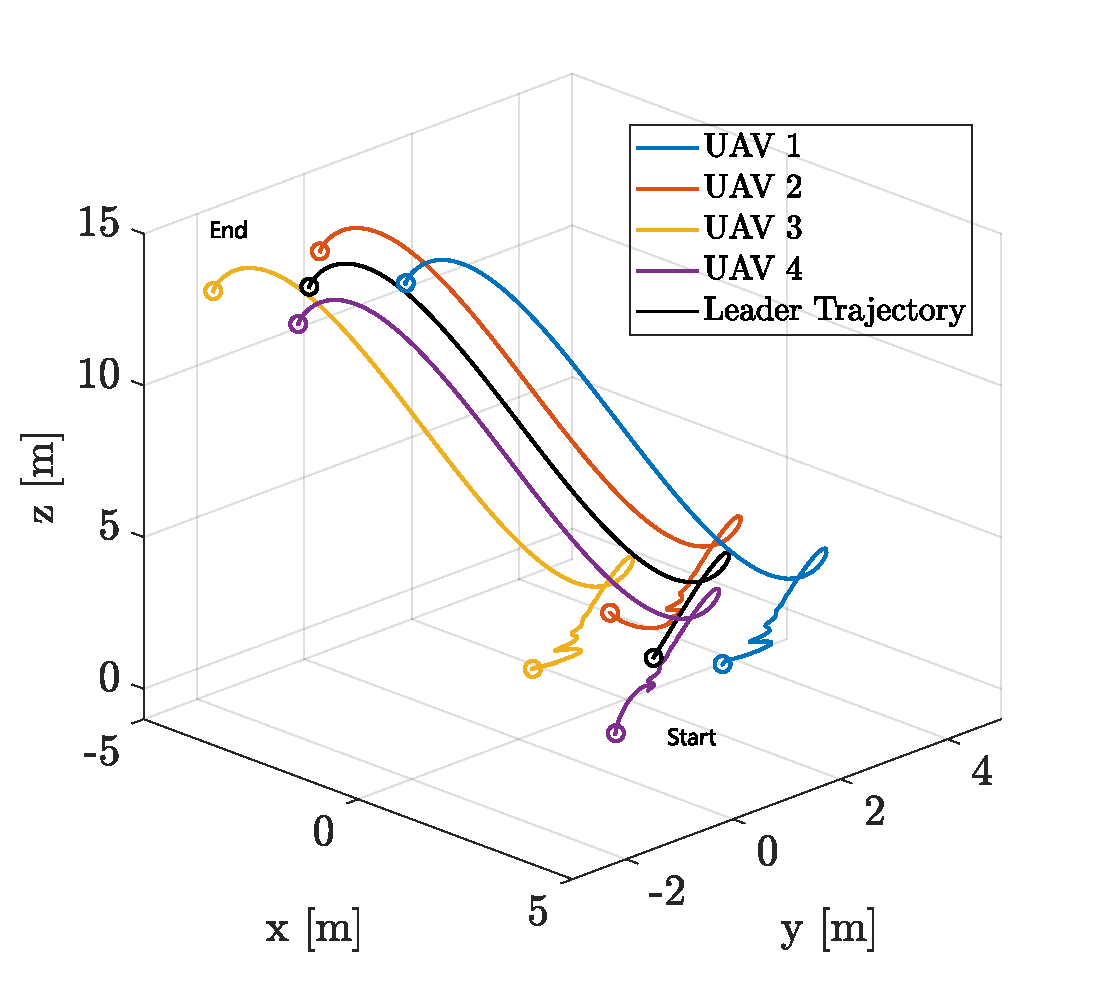
\includegraphics[width=0.8\textwidth]{Thesis_ICD/figure5/fig3dd.pdf}
    \caption{3-D formation trajectories of the UAVs.}
    \label{fig:3Dformation}
\end{figure}

A more detailed analysis is provided by the tracking error plots. Figure \ref{fig:err_pos} displays the position tracking errors for each UAV. The initial large errors, resulting from the dispersed starting positions, are quickly driven to a small neighborhood of the origin. Transient spikes are observable at $t=15s$ and $t=30s$ due to the topology switches, and a more pronounced spike is seen  at $t=25s$ and $t=35s$upon fault injection. However, in all cases, the controller rapidly suppresses these errors, demonstrating its robustness.

\begin{figure}[h!]
    \centering
    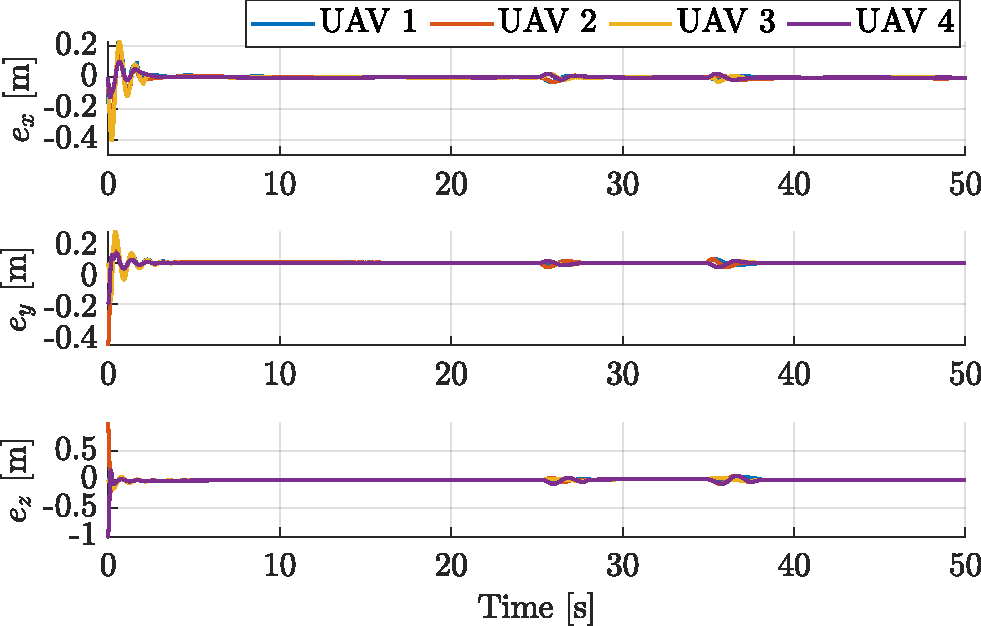
\includegraphics[width=0.8\textwidth]{Thesis_ICD/figure5/err_pos.pdf}
    \caption{Position tracking errors under actuator fault.}
    \label{fig:err_pos}
\end{figure}
 Similarly, Figure \ref{fig:err_vel} shows the velocity tracking errors, which also exhibit fast convergence and effective rejection of disturbances and faults.
\begin{figure}[h!]
    \centering
    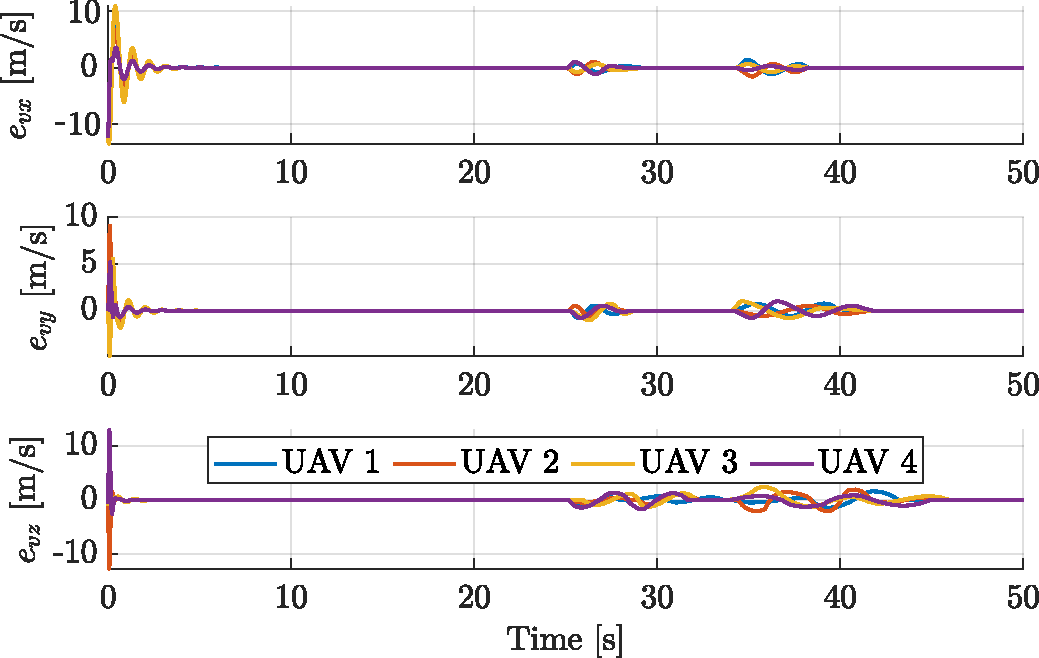
\includegraphics[width=0.8\textwidth]{Thesis_ICD/figure5/err_vel.pdf}
    \caption{Velocity tracking errors under actuator fault.}
    \label{fig:err_vel}
\end{figure}

\begin{figure}[h!]
    \centering
    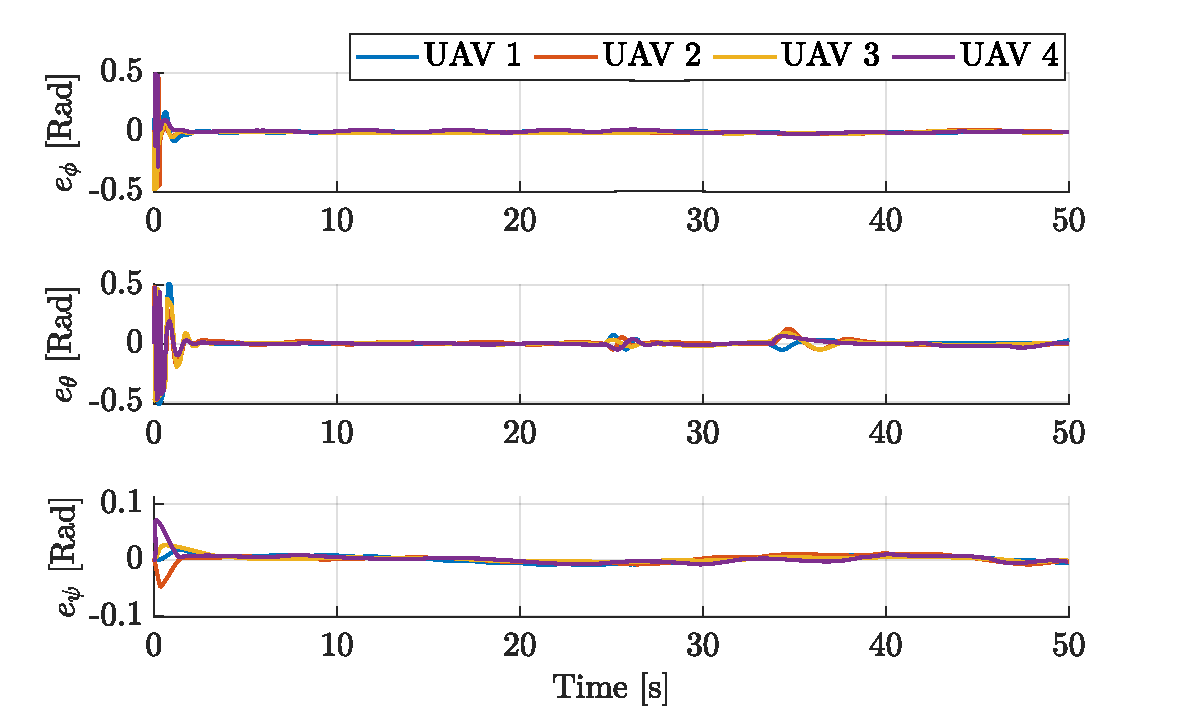
\includegraphics[width=0.8\textwidth]{Thesis_ICD/figure5/err_att.pdf}
    \caption{Attitude tracking errors under actuator fault.}
    \label{fig:err_att}
\end{figure}

The attitude tracking errors  follow a similar pattern of rapid convergence in Figure \ref{fig:err_att}, ensuring the UAVs maintain the correct orientation. The corresponding control inputs are shown in Figure \ref{fig:inputs}. The signals  remain within reasonable bounds, indicating the absence of chattering. The control input compensates for the actuator fault, confirming the successful operation of the adaptive SSNN estimator.

\begin{figure}[h!]
    \centering
    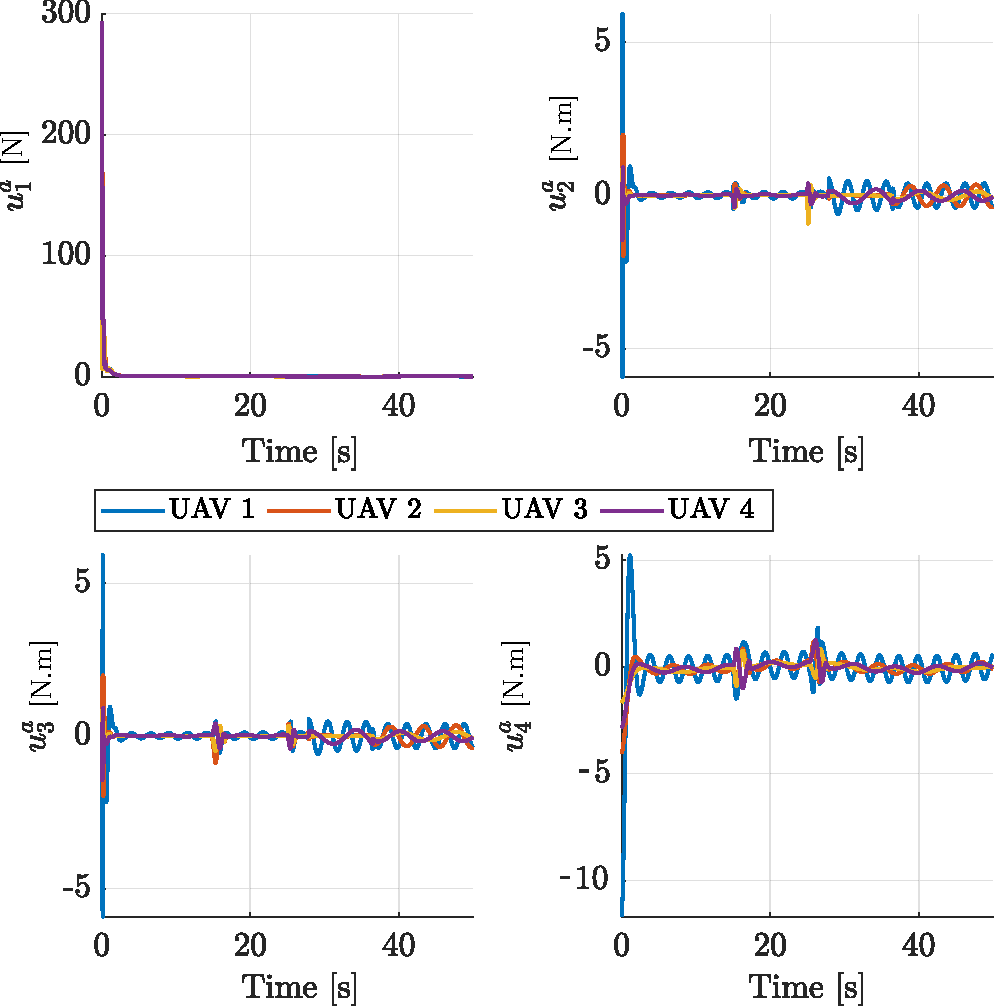
\includegraphics[width=0.8\textwidth]{Thesis_ICD/figure5/input.pdf}
    \caption{Control inputs of the UAVs.}
    \label{fig:inputs}
\end{figure}

To highlight the specific advantages of the proposed fixed-time control method, a performance comparison is conducted for UAV 3 against a standard sliding mode controller under the same conditions. Figures \ref{fig:fxtftpos} and \ref{fig:fxtftvel} show the position and velocity tracking errors for both controllers. The results clearly demonstrate that the proposed fixed-time controller (blue line) achieves a significantly faster convergence rate and a smaller steady-state error compared to its counterpart (orange line). This empirically validates the theoretical claim that the fixed-time stability approach provides superior performance in terms of both convergence speed and precision, which are critical for ensuring the safety and mission success of cooperative multi-UAV operations.

\begin{figure}[h!]
    \centering
    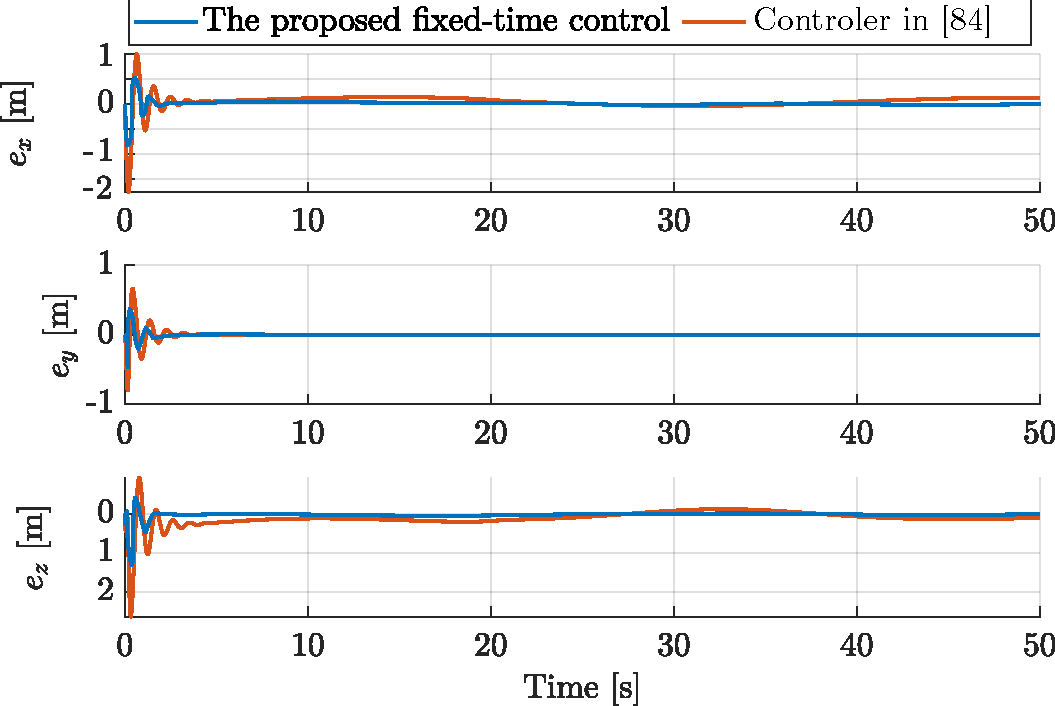
\includegraphics[width=0.8\textwidth]{Thesis_ICD/figure5/fxtftpos.pdf}
    \caption{Position tracking errors of UAV3.}
    \label{fig:fxtftpos}
\end{figure}

\begin{figure}[h!]
    \centering
    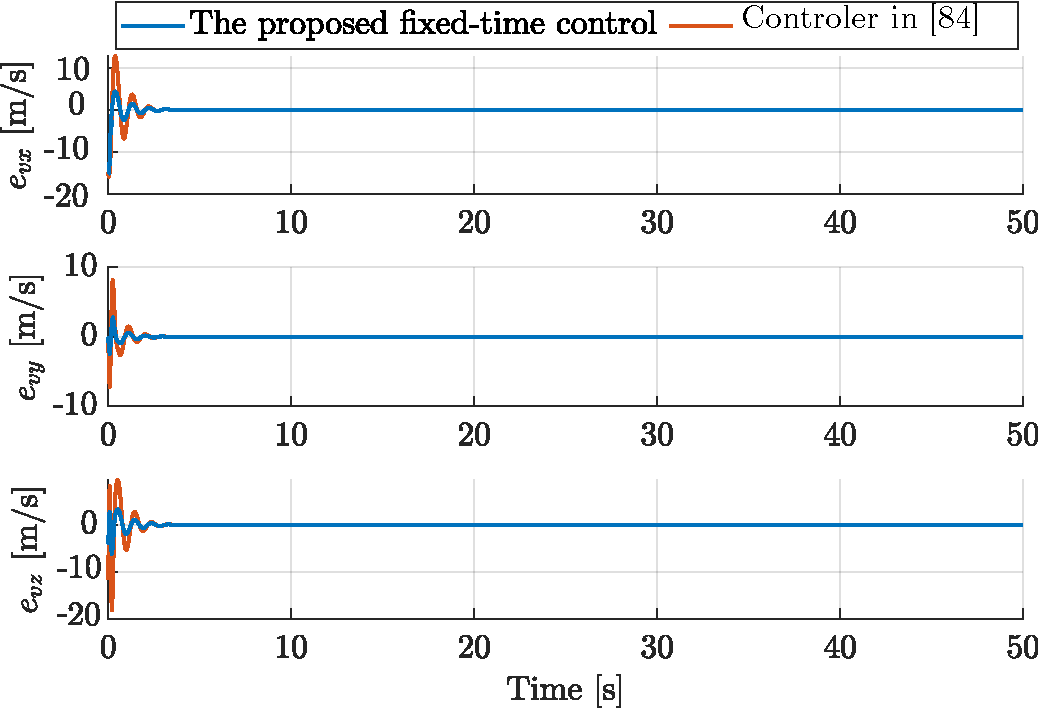
\includegraphics[width=0.8\textwidth]{Thesis_ICD/figure5/fxtftvel.pdf}
    \caption{Velocity tracking errors of UAV3.}
    \label{fig:fxtftvel}
\end{figure}

\section{Summary}
\label{sec5:conc}
This chapter addressed the distributed fault-tolerant formation control problem
for a group of coaxial rotor UAVs operating under actuator faults, external
disturbances, and switching communication topologies. The coaxial rotor platform
was selected for its aerodynamic efficiency and compact structure, while its
strongly coupled dynamics and inter-rotor interference made the control design
a genuine challenge, especially in the presence of faults.

The proposed framework was built on two main layers. The first is a distributed
formation protocol that generates desired trajectories for each follower UAV
based only on local neighbor information, ensuring that the entire group tracks
the virtual leader and maintains the prescribed geometric formation even as the
communication topology changes. The second is an individual fault-tolerant
controller designed for each UAV, combining a fixed-time sliding mode surface
with a Self-Structuring Neural Network (SSNN) that approximates and compensates
online for lumped uncertainties and actuator loss-of-effectiveness faults,
without requiring any prior training data. The SSNN dynamically grows or prunes
its own structure during operation, keeping the estimation accurate while
limiting the computational load on the onboard processor.

The stability of the closed-loop system was rigorously analyzed using Lyapunov
theory. It was shown that the formation tracking errors and the individual
position and attitude tracking errors all converge to a small bounded region
around the origin within a settling time $T_{\max}$ that is independent of the
initial conditions, satisfying the practical fixed-time stability requirement.
Simulation results confirmed the effectiveness of the proposed strategy under
simultaneous actuator faults, switching topologies, and external disturbances,
and demonstrated its clear advantage over a standard sliding mode controller
in terms of convergence speed and steady-state precision.

The contributions of this chapter complete the fault-tolerant control framework
developed throughout this thesis, extending it from single-vehicle systems to
the more complex and practically relevant setting of cooperative multi-UAV
formations. The general conclusions drawn from all chapters, along with
perspectives for future research, are presented in the following chapter.


